\begin{figure}[!htb]
  \centering
  \begin{subfigure}{0.08\textwidth}
    \centering
    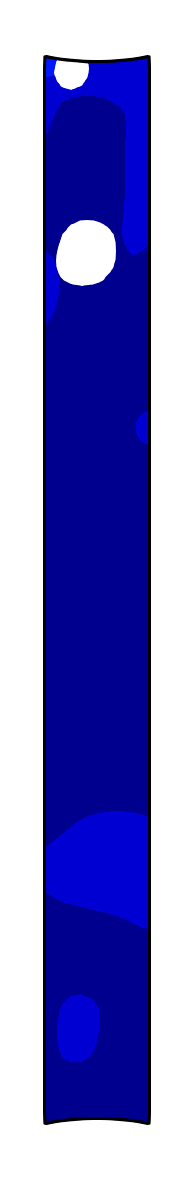
\includegraphics[width=\textwidth]{Chapter5/figures/spallation/psie_1}
  \end{subfigure}
  \begin{subfigure}{0.08\textwidth}
    \centering
    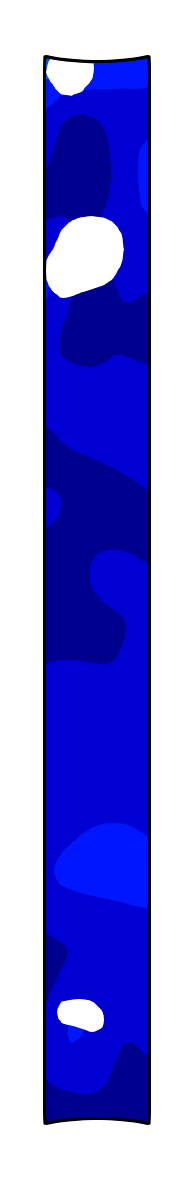
\includegraphics[width=\textwidth]{Chapter5/figures/spallation/psie_2}
  \end{subfigure}
  \begin{subfigure}{0.08\textwidth}
    \centering
    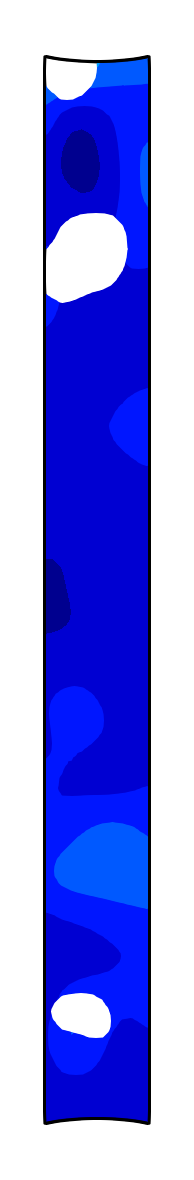
\includegraphics[width=\textwidth]{Chapter5/figures/spallation/psie_3}
  \end{subfigure}
  \begin{subfigure}{0.08\textwidth}
    \centering
    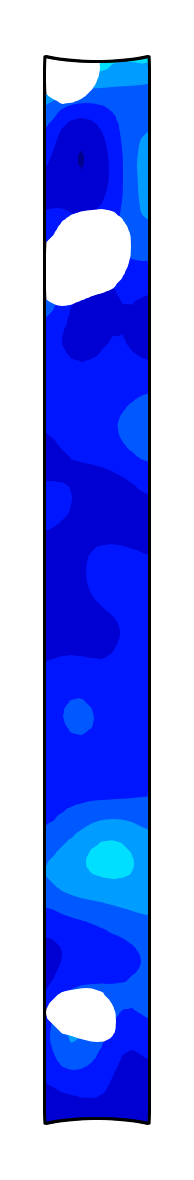
\includegraphics[width=\textwidth]{Chapter5/figures/spallation/psie_4}
  \end{subfigure}
  \begin{subfigure}{0.08\textwidth}
    \centering
    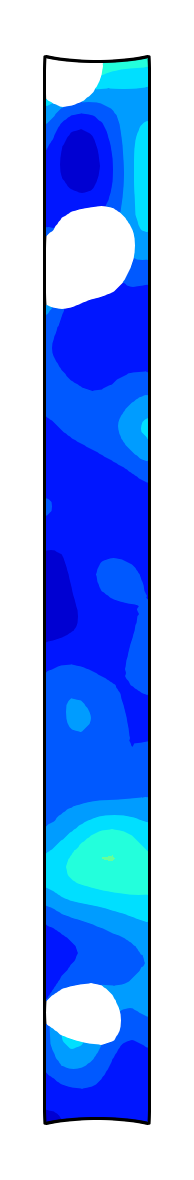
\includegraphics[width=\textwidth]{Chapter5/figures/spallation/psie_5}
  \end{subfigure}
  \begin{subfigure}{0.08\textwidth}
    \centering
    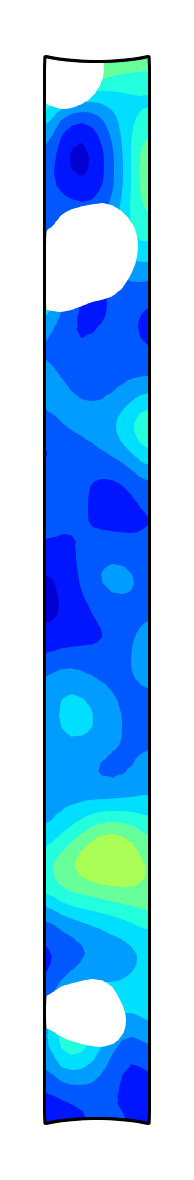
\includegraphics[width=\textwidth]{Chapter5/figures/spallation/psie_6}
  \end{subfigure}
  \begin{subfigure}{0.08\textwidth}
    \centering
    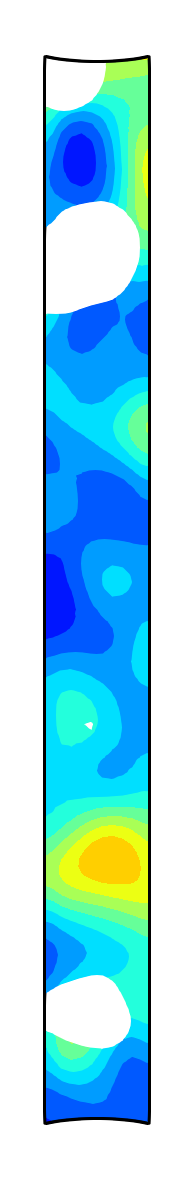
\includegraphics[width=\textwidth]{Chapter5/figures/spallation/psie_7}
  \end{subfigure}
  \begin{subfigure}{0.08\textwidth}
    \centering
    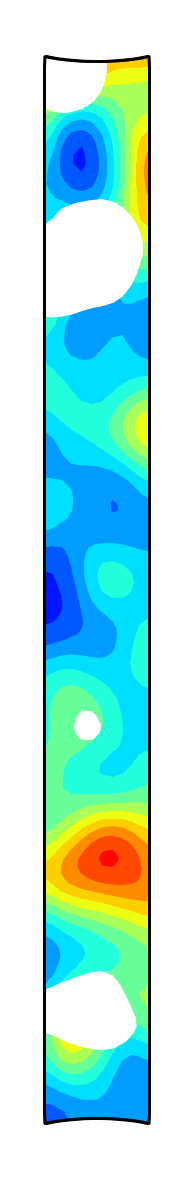
\includegraphics[width=\textwidth]{Chapter5/figures/spallation/psie_8}
  \end{subfigure}
  \begin{subfigure}{0.08\textwidth}
    \centering
    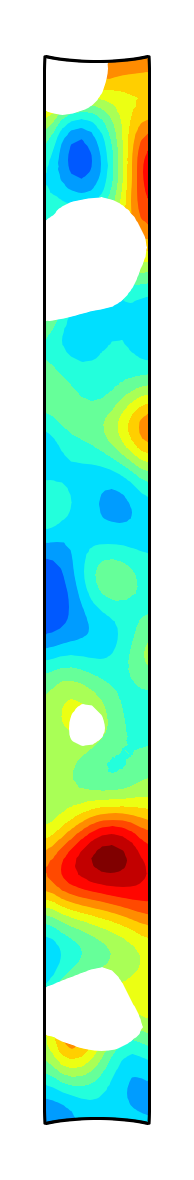
\includegraphics[width=\textwidth]{Chapter5/figures/spallation/psie_9}
  \end{subfigure}
  \begin{subfigure}{0.08\textwidth}
    \centering
    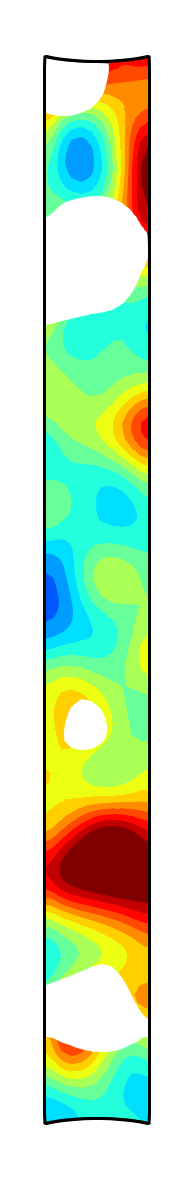
\includegraphics[width=\textwidth]{Chapter5/figures/spallation/psie_10}
  \end{subfigure}
  \begin{subfigure}{0.1\textwidth}
    \centering
    \caption*{$\psi^e_\activepart$}
    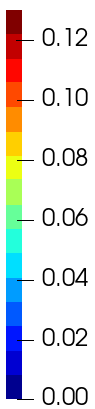
\includegraphics[width=0.8\textwidth]{Chapter5/figures/spallation/colorbar_psie}
  \end{subfigure}
  \caption{The active strain energy density right after each shut-down event. The region within the contour of $d = 0.75$ is removed to visualize in-plane fracture.}
  \label{fig: Chapter5/spallation/animation_psie}
\end{figure}
